\newcommand{\erdatamodaler}{ERwin Data Modeler~}

\chapter{Создание логической и физической модели данных}
\label{cha:dmd}
В данном разделе будет рассмотрено создание логической и физической модели данных предложенных предметных областей в ПО ERwin Data Modeler.

%На этапе инфологического проектирования базы данных должна быть построена
%модель предметной области, не привязанная к конкретной СУБД, понятная не только
%разработчикам информационной системы, но и экономистам, менеджерам и другим
%специалистам. В то же время модель предметной области должна максимально точно
%отражать семантику предметной области и позволять легко перейти к модели данных
%конкретной СУБД.
%
%\textbf{Логический уровень} --- это уровень, соответствующий инфологическому этапу проектирования
%и не привязанный к конкретной СУБД. Модели логического уровня оперируют с
%понятиями сущностей, атрибутов и связей, которые на этом уровне именуются на
%естественном языке (в нашем случае – на русском) так, как они называются в
%реальном мире.
%
%\textbf{Физический уровень} --- это отображение логической модели на модель данных
%конкретной СУБД. Одной логической модели может соответствовать несколько
%физических моделей. Причем, Erwin (как и другие CASE-системы проектирования баз
%данных) позволяет автоматизировать отображение логической модели на физическую.

\section{Работа по методическим указаниям}

Порядок построения модели данных в среде \erdatamodaler рассмотрим на примере
автоматизированной информационной системы <<Реализация средств вычислительной
техники>>, предназначенной для учета продаж настольных компьютеров по заказам
клиентов.

Создание модели данных начинается с разработки логической модели, которая
должна представлять состав сущностей предметной области с перечнем атрибутов и
отношений между ними.

\subsection{Построение модели данных}
Результат разработки логической модели данных системы <<Реализация средств
вычислительной техники>>, предназначенной для учета продаж настольных
компьютеров по заказам клиентов приведен на Рисунке \ref{fig:2-logical-model-method}.

% TODO: \usepackage{graphicx} required
\begin{figure}[htpb]
	\centering
	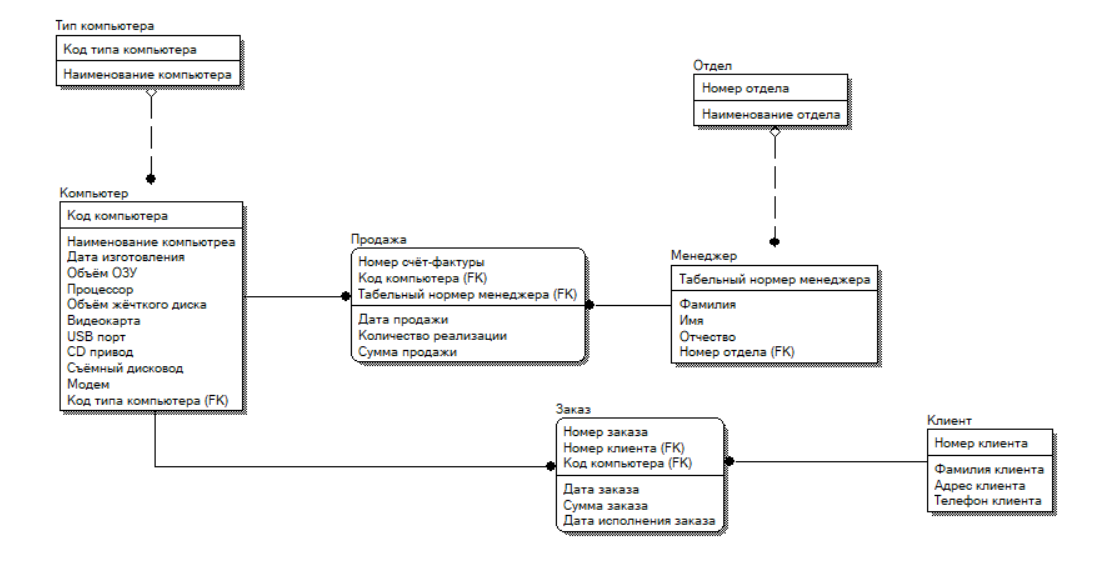
\includegraphics[angle=0,width=0.8\linewidth]{/2-method}
	\caption{Логическая модель данных системы <<Реализация средств вычислительной техники>>}
	\label{fig:2-logical-model-method}
\end{figure}

Для построения физической модели данных системы, следует определиться с СУБД, в которой будет реализована модель. При построении физической модели данных следует учитывать формальную теория представления и обработки данных в конкретной системе управления базами данных (СУБД).

В данной практической работе в качестве СУБД выбрана MySQL.

Приступим к построению физической модели данных системы <<Реализация средств вычислительной техники>>. Результат работы можно видеть на Рисунке \ref{fig:2-phisical-model}.
%\newpage
% TODO: \usepackage{graphicx} required
\begin{figure}[ht]
	\centering
	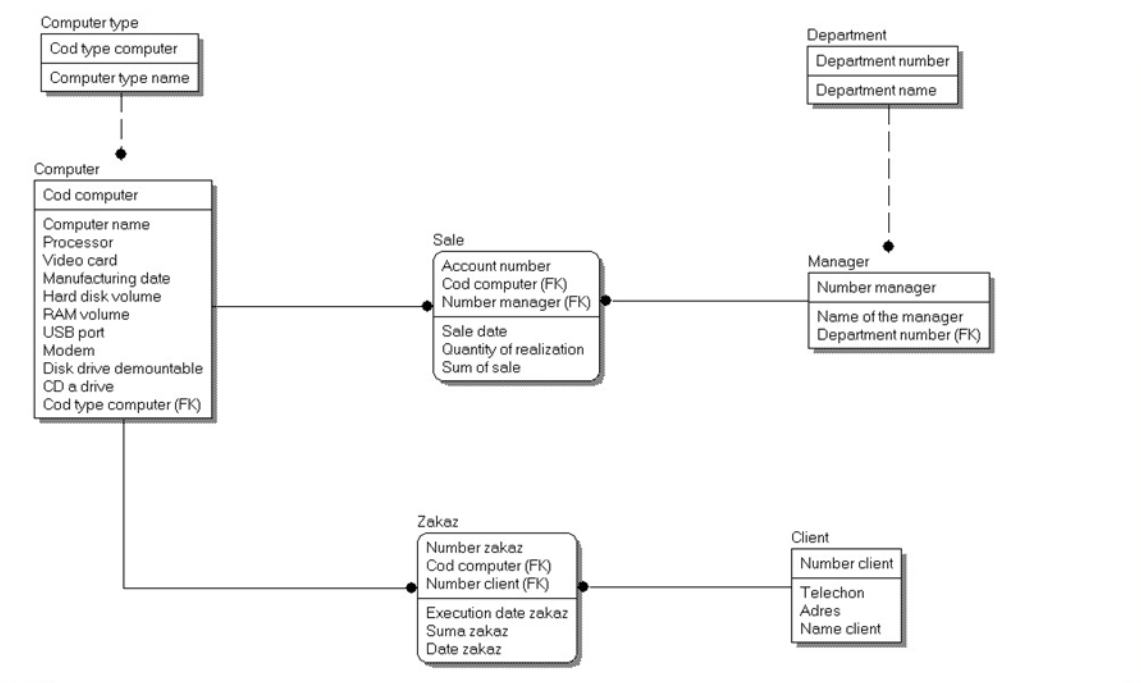
\includegraphics[angle=0,width=0.8\linewidth]{2-phisical-model}
	\caption{Физическая модель данных системы <<Реализация средств вычислительной техники>>}
	\label{fig:2-phisical-model}
\end{figure}
\newpage
\section{Индивидуальное задание}
Приступим к построению логической модели данных системы <<Велосипедное предприятие>>. 
В соответствии с моделью, реализованной в ходе первой практической работы, добавим в рабочую область следующие сущности:
\begin{itemize}
	\item Component;
	\item FrameInfo;
	\item Frame;
	\item Frameset;
	\item FrameSize;
	\item Fork;
	\item ComponentType;
	\item Wheelset;
	\item Groupset;
	\item Brake;
	\item FctCycleBuild;
	\item CycleType;
	\item Bar;
	\item Setup.
\end{itemize}
Добавим связи между сущностями в соответствии с ранее построенной моделью. Логическая модель системы <<Велосипедное предприятие>> приведена на Рисунке \ref{fig:2-cycle-logical}.

% TODO: \usepackage{graphicx} required
\begin{figure}[h!]
	\centering
	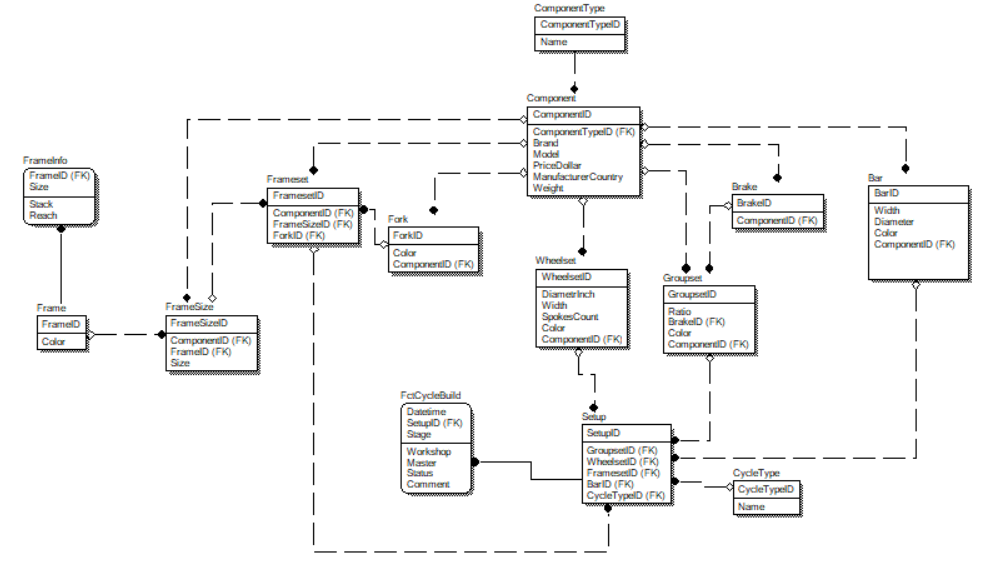
\includegraphics[width=0.8\linewidth]{2-cycle-logical}
	\caption{Логическая модель данных системы <<Велосипедное предприятие>>}
	\label{fig:2-cycle-logical}
\end{figure}
\newpage

\subsection{Построение модели данных}
После уточнения типов данных, выбранных в соответствии с предметной областью и спецификой СУБД MySQL.
Физическая модель системы <<Велосипедное предприятие>> приведена на Рисунке \ref{fig:2-cycle-phisical}.

% TODO: \usepackage{graphicx} required
\begin{figure}[h!]
	\centering
	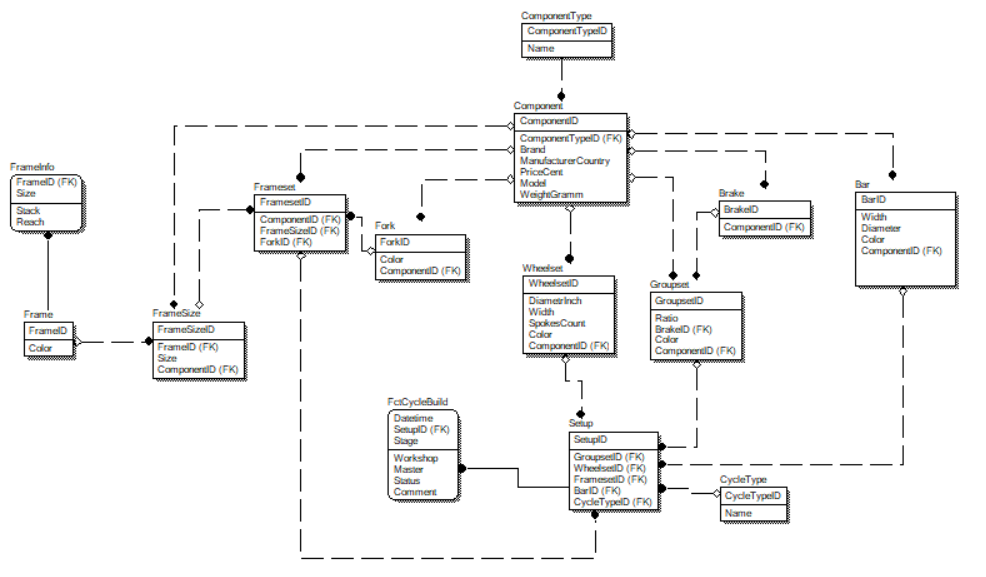
\includegraphics[width=0.8\linewidth]{2-cycle-phisical}
	\caption{Физическая модель данных системы <<Велосипедное предприятие>>}
	\label{fig:2-cycle-phisical}
\end{figure}

После реализации физической и логической модели можно приступать к реализации модели данной системы в СУБД MySQL.

\clearpage